\documentclass[12pt]{article}


% Language setting
% Replace `english' with e.g. `spanish' to change the document language
\usepackage[english]{babel}

% Set page size and margins
% Replace `letterpaper' with `a4paper' for UK/EU standard size
\usepackage[letterpaper,top=2cm,bottom=2cm,left=2cm,right=2cm,marginparwidth=2cm]{geometry}

\usepackage{listings}

% Useful packages
\usepackage{amsmath}
\usepackage{graphicx}
\usepackage[colorlinks=true, allcolors=blue]{hyperref}

\title{Polytechnique Montreal \\
LOG8415: Lab 1\\
Cluster Benchmarking using EC2 Virtual
Machines and Elastic Load Balancer (ELB)}

\author{Line Ghanem - 1728134\\Zineddine Aliche - 1949905\\
Mohammed Ramzi Bouthiba - 2065386\\Axelle Pagnier - 2164162}

\begin{document}
\maketitle

\begin{abstract}
In	assignment,	we	will	create	two	clusters of	EC2 virtual	machines and use	load	balancer	to	distribute	workloads	and	perform	extensive	benchmarking	on	those instances.\newline
First we will explain the overall architecture that is going to be deployed using Amazon Web Services. Then we will talk about the flask application that we deployed on the EC2 instances. After that, we will discuss the performance metrics of the instances and the load balancer that we retreived using CloudWatch.	Finally, we will provide an automated solution to do the set up and the benchmarking.
\end{abstract}

\section{Setting Up the Environment}
In this section, we discuss the steps that lead to the creation of instances, target groups and the load balancer in order to prepare our environment to receive the tasks requested in this laboratory.Figure 1 illustrates the path we followed to setting up the environment.\\
We start with the creation of a custom core virtual networking with the Amazon virtual Private Cloud (VPC) service, the goal is to have complete control of the virtual network environment, including resource placement, connectivity, and security.\\
The second step consists in the creation of an internet gateway which allows to ensure the communication between our resources in the VPC and the internet.\\
The creation of a custom VPC needs to have custom subnets, for this we have created two different subnets, one for each availability zone ('us-east-1a' and 'us-east-1b'), but before creating the subnets we have established a routing table because each subnet in VPC must be associated with a routing table, which controls the network traffic routing for the subnet.\\
To secure the instances that we are going to generate, we have created a security group which acts as a virtual firewall for our EC2 instances and which contains a set of rules that filter incoming and outgoing traffic.\\
Once all the steps discussed above have been completed, we proceed to the creation of our EC2 instances, in total \textbf{9} instances have been created in the same region \textbf{'us-east-1'}, with two different types of instances: \textbf{'m4.large'} and \textbf{'t2.large'}. Five (05) of the instances are of type 'm4.large' in the availability zone 'us-east-1a' and four (04) are of type 't2.large' in the availability zone 'us-east-1b'.\\
In order to group the instances to form the clusters, two target groups have been made, the first with the instances of type 'm4.large' and the second with the type 't2.large'.\\
The final step for setting up the environment is the creation of the load balancer, which will manage the request traffic sent to our clusters, the type of load balancer used is \textbf{Application Load Balancer} (ALB) that operate at layer 7 (application layer).



\begin{figure}[h]
  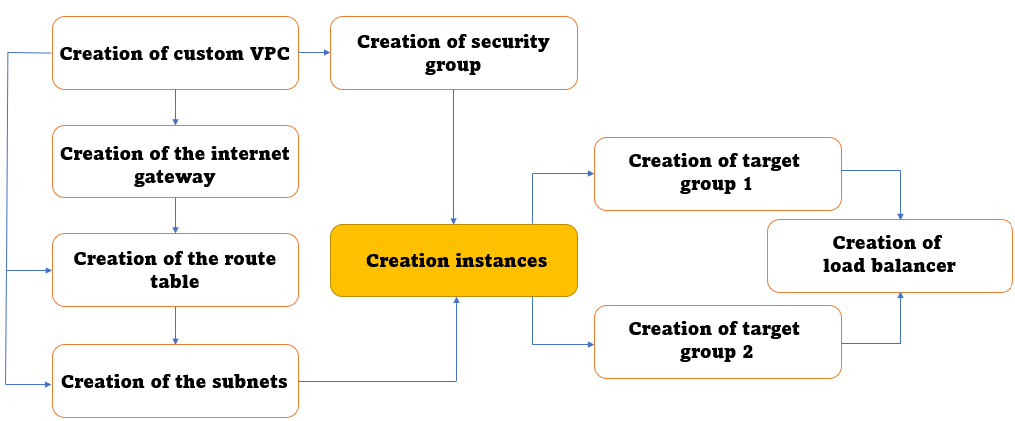
\includegraphics[width=\linewidth]{Environment_setup.png}
  \caption{Setting up the environment.}
  \label{fig:boat1}
\end{figure}

\section{Deploying the Flask Application}
To deploy the flask application we created an ssh connection to each of the instances using the python library paramiko \cite{paramiko}. 
Once the connection was established using the key pair we ran a bash script that would set up the environment for python and flask, add the code for the application and then deploy it on port 80 of each instance. 
\\
To deploy our small app we simply used:
\begin{lstlisting}[language=Bash]
nohup sudo flask run --host=0.0.0.0 --port=80 1>/dev/null 2>/dev/null &
\end{lstlisting}
The bash command \emph{nohup}, keeps any process that is started after it running in the background so that we can exit the command line safely without stopping our small app. For example, given an instance with a public ip: 111.111.111, the user can go to the following url: http://111.111.111:80 and the app should be running. The page should simply display a message: \\
\emph{Your small app is working on instance id: instance\_id}.\\ It is important in the following assignment to know which instance is responding since we will try to connect to the website using the load balancer. 

\section{Benchmarking}
\section{Conclusion}

\begin{thebibliography}{9}
\bibitem{paramiko}
Paramiko, Availible online: https://www.paramiko.org/, Accessed: Oct. 2022. 
\end{thebibliography}

\end{document}